%%%%%%%%%%%%%%%%%%%%%%%%%%%%%%%%%%%%%%%%%%%%%%%%%%%%%%%%%%%%%%%%%%%%%%
%% Springer Nature LaTeX template (v3.1).                             %%
%% Two-column layout: the `iicol' class option.                       %%
%% To return to the single-column layout, delete `iicol' below.        %%
%%                                                                    %%
%% Build with pdfLaTeX (the engine named by the `pdflatex' option):    %%
%%   pdflatex AspectStance; bibtex AspectStance;                       %%
%%   pdflatex AspectStance; pdflatex AspectStance                      %%
%% XeLaTeX is not supported: under it the class sets figure captions   %%
%% with incorrect (about 13 pt) leading.                               %%
%%%%%%%%%%%%%%%%%%%%%%%%%%%%%%%%%%%%%%%%%%%%%%%%%%%%%%%%%%%%%%%%%%%%%%

\documentclass[pdflatex,sn-mathphys-num,iicol]{sn-jnl}% Math and Physical Sciences Numbered Reference Style, two columns

%%%% Standard packages
\usepackage{graphicx}%
\usepackage{amsmath,amssymb,amsfonts}%
\usepackage[table]{xcolor}%
\usepackage{textcomp}%
\usepackage{booktabs}%
\usepackage[most]{tcolorbox}%
\usepackage{ragged2e}
\usepackage{array}
\usepackage{tabularx}
\usepackage{dblfloatfix}% robust placement for page-wide floats
\usepackage{microtype}% tighter line filling, fewer stretched columns
%%%% Let URLs break after any lower-case letter, so that narrow columns are not stretched
\makeatletter
\AtBeginDocument{\g@addto@macro\UrlBreaks{\do\a\do\b\do\c\do\d\do\e\do\f\do\g\do\h\do\i\do\j\do\k\do\l\do\m\do\n\do\o\do\p\do\q\do\r\do\s\do\t\do\u\do\v\do\w\do\x\do\y\do\z}}
\makeatother
\hypersetup{
	bookmarksdepth=2,
	pdftitle={AspectStance: Unsupervised Discovery of Target-Specific Aspects for Stance Detection},
	pdfauthor={Milad Allahgholi and Hossein Rahmani},
	pdfsubject={Target-level stance detection conditioned on unsupervised, target-specific aspect discovery},
	pdfkeywords={stance detection, unsupervised aspect discovery, LLM-based text enrichment, K-means clustering, social media}
}

%%%% Table column types
\newcolumntype{Y}{>{\RaggedRight\arraybackslash}X}
\newcolumntype{C}[1]{>{\centering\arraybackslash}m{#1}}
\newcolumntype{M}[1]{>{\raggedright\arraybackslash}m{#1}}
\newcolumntype{L}[1]{>{\RaggedRight\arraybackslash}p{#1}}

%%%% Table styling: shaded band rows for group/target headings
\definecolor{snband}{HTML}{E6EDF5}
\definecolor{snaccent}{HTML}{2F6DB5}
\definecolor{snrule}{HTML}{A9BACB}
\definecolor{snbox}{HTML}{F6F8FB}
%%%% Band overhang: 0pt for tables with @{} at both edges; \tabcolsep for tables with edge padding
\newlength{\bandoverhang}\setlength{\bandoverhang}{0pt}
\newcommand{\bandstrut}{\rule[-0.8ex]{0pt}{3.2ex}}
\newcommand{\tabband}[2]{%
  \rowcolor{snband}[\bandoverhang][\bandoverhang]\multicolumn{#1}{@{}l@{}}{\bandstrut#2}\\}

%%%% Share bar for the inventory tables: bar length proportional to the share
\newlength{\sbarunit}\setlength{\sbarunit}{0.021cm}
\newcommand{\sbar}[1]{\textcolor{snaccent!75}{\rule[-0.12ex]{#1\sbarunit}{1.3ex}}}
%%%% Across-run standard deviation, set after a mean (6.5 pt beside the 8 bp table text)
\newcommand{\sd}[1]{{\fontsize{6.5}{7.5}\selectfont$\pm$#1}}
%%%% Inventory-table helper: one heading row per target
\newcommand{\aspecthead}[3]{%
  \tabband{4}{\textsc{#1}\quad\textnormal{$K=#2$,\ Sil.\ #3}}}
%%%% Braces inside the typewriter prompt boxes: take them from the typewriter font
%%%% (with OT1 encoding, \{ and \} would fall back to the math symbol font)
\newcommand{\ttlbrace}{\char`\{}
\newcommand{\ttrbrace}{\char`\}}

\makeatletter%
%%%% Float separations, slightly tighter than the class defaults (15--20 pt)
%%%% but large enough to separate floats clearly from the running text.
%%%% Display-math skips are left to the class (\normalsize resets them).
\AtBeginDocument{%
	\setlength{\textfloatsep}{12pt \@plus 3pt \@minus 2pt}%
	\setlength{\dbltextfloatsep}{12pt \@plus 3pt \@minus 2pt}%
	\setlength{\floatsep}{10pt \@plus 2pt \@minus 2pt}%
	\setlength{\dblfloatsep}{10pt \@plus 2pt \@minus 2pt}%
	\setlength{\intextsep}{10pt \@plus 2pt \@minus 2pt}%
	\setlength{\abovecaptionskip}{6pt}%
	\setlength{\belowcaptionskip}{4pt}%
}
\makeatother%
%%%% Float placement: the inventories and examples use page-wide floats.
\renewcommand{\topfraction}{0.92}
\renewcommand{\bottomfraction}{0.75}
\renewcommand{\textfraction}{0.10}
\renewcommand{\floatpagefraction}{0.72}
\renewcommand{\dbltopfraction}{0.9}
\renewcommand{\dblfloatpagefraction}{0.7}
\setcounter{topnumber}{3}
\setcounter{totalnumber}{4}
\setcounter{dbltopnumber}{3}

\raggedbottom
\clubpenalty=10000
\widowpenalty=10000
\displaywidowpenalty=10000

\begin{document}

\title[AspectStance]{AspectStance: Unsupervised Discovery of Target-Specific Aspects for Stance Detection}

\author[1]{\fnm{Milad} \sur{Allahgholi}}\email{milad\_allahgholi@comp.iust.ac.ir}

\author*[1]{\fnm{Hossein} \sur{Rahmani}}\email{h\_rahmani@iust.ac.ir}

\affil[1]{\orgdiv{School of Computer Engineering}, \orgname{Iran University of Science and Technology}, \orgaddress{\city{Tehran}, \country{Iran}}}

\abstract{Stance detection identifies the attitude of a social media post towards a target such as a politician or a social issue. Most methods assign one label to the whole target and leave implicit which aspect of it, such as a policy or event, a post addresses. We propose \textit{AspectStance}, which discovers target-specific aspects without annotation and uses them to condition a supervised stance classifier. For each post, a large language model (\textit{GPT-6 Luna}) writes a short gloss relating it to the target. The post and gloss are embedded separately, reduced with UMAP fitted on the training posts, and concatenated. K-means groups these vectors into aspect clusters, a silhouette sweep sets the cluster count for each target, and new posts are routed to the nearest frozen centroid. A classifier ensemble then predicts stance from the post representation and a one-hot aspect encoding. Averaged over ten seeded runs, \textit{AspectStance} reaches a target-averaged \textsc{favor}/\textsc{against} F1 of 90.8 on P-Stance and 85.3 on SemEval-2016 Task~6, 10.1 and 15.7 points above the same ensemble without the aspect feature, with gains on all eight targets. Replacing K-means with random clustering lowers the scores by 15.1 and 11.2 points, even when each target keeps its best of 160 random configurations on the test split. Most discovered aspects correspond to recognisable subtopics, such as impeachment or abortion legislation. Although each aspect is derived from information the classifier already receives, the results indicate that making it explicit provides a useful inductive bias. The implementation is available at \url{https://github.com/miladallahgholi95/AspectStance}.}

\keywords{Stance detection, Unsupervised aspect discovery, LLM-based text enrichment, K-means clustering, Social media}

\maketitle

\section{Introduction}\label{sec1}

A post about a presidential candidate is rarely about the candidate in general. More often, it concerns a debate performance, a health-care proposal, a fundraising appeal, or a scandal. Stance detection nonetheless asks for a single verdict on the target as a whole: \textsc{favor}, \textsc{against}, or \textsc{none} \cite{alturayeif2023systematic,kucuk2020stance}. Analyses of political debate and online public opinion rely on this label \cite{burnham2025stance,cao2022stance,aldayel2021stance}. Neural and large language model (LLM) methods have steadily improved the representations behind this decision \cite{gera2025deep}, but the label still collapses distinct arguments: criticism of a candidate's economic policy and criticism of their personal conduct both reduce to \textsc{against}.

Recovering these distinctions requires knowing which aspect of the target a post addresses. Standard benchmarks annotate only the target, so the aspect under discussion is never recorded. Topic-aware stance methods try to recover this information in different ways \cite{gomez2023stance,li2023stance,cheng2024cosd,muthusami2025interpretable}. They differ in where topics are induced, whether stance labels guide the induction, how the number of topics is chosen, and how topic structure reaches the predictor. We ask a narrower question: if the posts of each target are grouped into aspects without aspect supervision, and each post's group is given directly to the classifier, does target-level stance detection improve?

To answer it, \textit{AspectStance} builds an inventory of latent aspects for each target, where each aspect is a cluster of posts. An LLM first writes a short gloss explaining how a post relates to its target. The post and the gloss are embedded, projected into a shared low-dimensional space, and concatenated, and K-means groups the resulting vectors, with a silhouette criterion choosing the number of clusters for each target. A small classifier ensemble then sees each post's vector together with a one-hot code for its cluster. At test time, the projection and the centroids stay frozen, so a new post is assigned by the same rule that grouped the training posts. Clusters are named afterwards, purely to make them readable; the names never enter the prediction.

The paper makes three contributions:
\begin{enumerate}
	\item We introduce \textit{AspectStance}, a pipeline that discovers a latent aspect inventory for each target without aspect annotation, conditions a supervised stance classifier on it, and returns the assigned aspect with every prediction.
	\item We test the cluster feature with a matched ablation and a clustering-strategy control. The cluster is computed from the post and its gloss, so it carries no information that the classifier does not already receive. Yet, with the rest of the pipeline held fixed, supplying it adds 10.1 F1 points on P-Stance and 15.7 on SemEval-2016 Task~6, and the mean gain over ten seeded runs is positive on all eight targets. Replacing K-means with random clustering, again with every other component unchanged, lowers the scores by 15.1 and 11.2 points, so the gain depends on the induced partition and not merely on the presence of a cluster feature.
	\item We analyse the discovered inventories and show which subtopics of each target the partition recovers.
\end{enumerate}
Table~\ref{tab:positioning} (Section~\ref{subsec25}) contrasts the design with closely related systems, and Section~\ref{subsec71} discusses why the explicit partition helps.

The experiments address four questions. \emph{RQ1.} Does cluster conditioning improve an otherwise matched target-level classifier? \emph{RQ2.} Is the gain consistent across targets and seeds? \emph{RQ3.} Does the gain depend on the clustering strategy, or would random clusters serve equally well? \emph{RQ4.} What thematic structure appears in the induced inventories? Section~\ref{sec2} reviews related work, and Sections~\ref{sec3}--\ref{sec5} define the task, describe the framework, and set out the evaluation protocol. Section~\ref{sec6} reports the results, Section~\ref{sec7} discusses them together with the limitations of the study, and Section~\ref{sec8} concludes.

\section{Related work}\label{sec2}

Prior work on stance detection spans feature-based classifiers, neural encoders, and LLMs. We review these strands briefly and then concentrate on topic- and aspect-aware methods, which are closest to \textit{AspectStance}.

\subsection{Feature-based approaches}\label{subsec21}
Feature-based stance detectors represent posts with n-grams, part-of-speech tags, lexicon scores, and dependency patterns, and classify these cues with support vector machines, naive Bayes, or logistic regression \cite{masood2018fake,ayyub2021stance}. Such cues are easy to inspect, but they must be redesigned whenever the topic or platform changes. Learned representations reduce the need for such redesign, but cross-target transfer and interpretability remain open problems \cite{alturayeif2023systematic,aldayel2021stance}.

\subsection{Neural and transformer-based approaches}\label{subsec22}
Neural stance detectors replace handcrafted features with learned lexical and contextual representations. Conditional encoding of text and target showed early on that the target should shape the representation rather than merely be appended to it \cite{augenstein2016stance}. Later work tests transfer through multi-dataset training \cite{schiller2021stance}, adds auxiliary supervision such as sentiment and sarcasm \cite{alturayeif2023enhancing}, and incorporates further signals, including hashtag enrichment for implicit stance \cite{dong2024implicit}, emotion-aware objectives \cite{pu2025integrating}, and target--stance graphs \cite{cai2025enhancing}. Cross-target and zero-shot studies examine transfer to sparsely labelled or unseen targets \cite{allaway2020zero,khiabani2025cross}. In all of these models, the aspect of the target that a post addresses remains largely implicit. \textit{AspectStance} stays within supervised in-target classification and makes this aspect an explicit input.

\subsection{Large language model approaches}\label{subsec23}
LLMs have been used both to predict stance directly and to generate contextual explanations. Studies of informal political discourse have examined how additional context changes these predictions \cite{gambini2024evaluating,sucu2025exploiting}. Other systems impose more structure on the reasoning, through chains of stance reasoning \cite{ma2024chain}, multiple reasoning paths \cite{zhang2025mprf}, multi-perspective verification \cite{zhang2025mpvstance}, or collaborating LLM agents with assigned analytical roles \cite{lan2024cola}. Context-aware zero-shot prompting adds generated context to the prompt itself \cite{allahgholi2025conspro}. A further line uses LLM-generated text as input to a supervised model: KASD enriches posts with LLM-processed background knowledge \cite{li2023stance}, and chain-of-thought embeddings pass an LLM's reasoning about a post to a supervised stance classifier \cite{gatto2023cot}. The gloss branch of \textit{AspectStance} belongs to this family.

Two recent zero-shot frameworks give LLM reasoning further structure. MSME \cite{zhang2026msme} assigns external knowledge, target--label relations, and pragmatic interpretation to separate expert components, and a cognitive inductive-reasoning approach \cite{zhang2026induce} derives schemas and aligns them through a graph. Both organise the reasoning process, but neither groups the posts of each target into aspects, which is the basis of \textit{AspectStance}.

\subsection{Topic- and aspect-aware approaches}\label{subsec24}
Topic-aware methods are the closest precedents, because they place a layer of thematic structure between the text and the stance decision.

G\'omez-Suta et al. \cite{gomez2023stance} use target-dependent topic features to support explainable stance classification. KASD \cite{li2023stance} fits latent Dirichlet allocation (LDA) \cite{blei2003latent} separately for each target, uses the resulting topics to retrieve background knowledge from Wikipedia, and has an LLM condense that knowledge and paraphrase the discourse of each post. The number of topics, between 5 and 19, is selected by the minimum first-order difference in perplexity. CoSD \cite{cheng2024cosd} induces topics for each target and stance-label subset and then constructs a heterogeneous topic graph. Aiming instead at transfer to unseen targets, Allaway and McKeown \cite{allaway2020zero} apply K-means to contextual representations of document--topic pairs and supply the resulting generalised topic representation to the classifier. Contrastive prototypes serve a related role in zero-shot stance detection \cite{liang2022jointcl}. Target-specific topic induction and a data-driven rule for inventory size already exist in this literature, most clearly in KASD. None of these stance methods, however, induces the partition from an LLM-written, target-conditioned gloss of each post, or returns the induced cluster with the prediction.

Muthusami et al. \cite{muthusami2025interpretable} combine BERTopic \cite{grootendorst2022bertopic} topic discovery with a RoBERTa classifier, incorporating topic assignments and sentiment information as features. Their combination of contextual embeddings, Uniform Manifold Approximation and Projection (UMAP), and clustering is especially close to our pipeline. Arakelyan et al. \cite{arakelyan2023topic} use topics in another role, for diversity sampling and contrastive learning, and do not output them at prediction time. Among shared tasks, SemEval-2026 Task~3 (DimABSA) includes dimensional stance analysis, which treats stance targets as aspects and predicts valence and arousal \cite{yu2026dimabsa}. These dimensional outputs differ from the categorical, target-level labels used here.

Outside stance detection, LLM-generated text has been used to shape the representation that a clustering algorithm receives. Viswanathan et al. \cite{viswanathan2024fewshot} concatenate the embedding of LLM-generated keyphrases with the document embedding before K-means, and IDAS \cite{deraedt2023idas} clusters utterances together with short LLM-written summaries to discover intents. \textit{AspectStance} applies this principle to stance detection: the generated text is conditioned on the stance target, the partition is induced separately for each target, and its clusters condition a supervised stance classifier.

The term \emph{aspect} comes from aspect-based sentiment analysis, where sentiment is predicted for annotated or extracted aspects of an entity \cite{pontiki2014semeval,zhang2023absasurvey}. Unsupervised aspect extraction discovers such aspects without annotation, for example by reconstructing sentence embeddings from a small set of learned aspect embeddings \cite{he2017unsupervised}. In \textit{AspectStance}, by contrast, an aspect is an induced cluster that conditions a single target-level stance label; it does not receive a polarity of its own. Aspect-like structure has also been studied as the reasons behind a stance \cite{hasan2014why} and as the key points that summarise the arguments on a topic \cite{barhaim2020keypoints}. Target-specific attention conditions a neural encoder on the target without inducing such structure \cite{du2017tan}. Finally, supplying cluster membership as an input feature is an established device in supervised learning, from word-cluster features \cite{turian2010word} to K-means feature learning \cite{coates2012kmeans}.

\subsection{Positioning of this work}\label{subsec25}
Table~\ref{tab:positioning} compares \textit{AspectStance} with the three closest precedents in terms of six design choices: the scope of topic induction, whether stance labels are used, whether LLM-generated text enters the pipeline, how the number of topics is set, what representation the topics are induced from, and what role they play at prediction time.

\begin{table*}[t]
	\caption{Design comparison of \textit{AspectStance} with closely related topic-aware stance detection methods. The columns correspond to six design choices that determine how thematic structure is induced and how it is used at prediction time.}
	\label{tab:positioning}
	\centering
	\setlength{\tabcolsep}{5pt}
	\renewcommand{\arraystretch}{1.2}
	\tablebodyfont\hyphenpenalty=10000\exhyphenpenalty=10000
	\begin{tabularx}{\textwidth}{@{}>{\hsize=1.05\hsize}Y >{\hsize=0.92\hsize}Y >{\hsize=0.70\hsize}Y >{\hsize=0.88\hsize}Y >{\hsize=1.18\hsize}Y >{\hsize=1.02\hsize}Y >{\hsize=1.25\hsize}Y@{}}
		\toprule
		\textbf{Method} & \textbf{Induction scope} & \textbf{Uses stance labels} & \textbf{LLM-\allowbreak generated text} & \textbf{Topic count set by} & \textbf{Topics induced from} & \textbf{Role at prediction time} \\
		\midrule
		KASD \cite{li2023stance} & Per target & No & Condensed knowledge and paraphrase & Minimum first-order perplexity difference, \mbox{$K=5,\ldots,19$} & Words, via LDA & Retrieval key for external knowledge \\
		\addlinespace[2pt]
		CoSD \cite{cheng2024cosd} & Per target and per stance-label subset & Yes & None & Fixed in advance & Words, via LDA & Nodes of a heterogeneous topic graph \\
		\addlinespace[2pt]
		Topic-guided transformer \cite{muthusami2025interpretable} & Per-target fitting not specified & Not for topic discovery & None & Implicitly, by HDBSCAN density clustering & Contextual embeddings, via BERTopic & Topic assignments as classifier features \\
		\addlinespace[2pt]
		\textbf{\textit{AspectStance}} & Per target & No & Per-post gloss & Maximum silhouette over 2--30 clusters & Post and gloss embeddings, via K-means & One-hot conditioning feature, returned with the label \\
		\bottomrule
	\end{tabularx}
\end{table*}

Unlike KASD and CoSD, \textit{AspectStance} clusters contextual embeddings and passes the cluster directly to the classifier. The topic-guided transformer shares both properties. Among stance detection methods, \textit{AspectStance} differs in three respects: it clusters each post together with its target-conditioned gloss, selects the inventory size by a silhouette sweep, and uses the resulting aspect as a one-hot conditioning feature that is returned with each prediction. Section~\ref{sec6} tests the cluster feature within this pipeline through a matched ablation and a clustering-strategy control.

\section{Problem formulation}\label{sec3}

Let \(T\) denote a \emph{target}, such as a person, a policy, or a social issue. For each target, we are given \(N_T\) labelled posts
\begin{equation}\label{eq:data}
\mathcal{D}_T = \{(x_i, y_i)\}_{i=1}^{N_T}, \qquad y_i \in \mathcal{Y}_T,
\end{equation}
where \(x_i\) is a post and \(y_i\) is its stance towards \(T\). The label set is \(\mathcal{Y}_T = \{\textsc{favor}, \textsc{against}\}\) for P-Stance; SemEval-2016 Task~6 adds \textsc{none}.

A standard target-level classifier learns a single mapping \(x \mapsto y\); the Base Method of Section~\ref{subsec53} has this form. \textit{AspectStance} inserts an intermediate variable between the post and its label: the \emph{aspect} \(c\) of the post, which is the index of one of \(K_T\) latent, target-specific aspects. No aspect labels are available, and \(K_T\) is unknown and may differ across targets. The task therefore becomes the following.

\begin{tcolorbox}[colframe=snrule, colback=snbox, boxrule=0.6pt, arc=3pt, width=\linewidth, left=6pt, right=6pt, top=4pt, bottom=5pt, before skip=8pt, after skip=8pt]
\textbf{Problem.} Given \(\mathcal{D}_T\) but no aspect labels, learn an aspect-assignment function and an aspect-conditioned stance classifier,
\begin{align}
h_T &: x \mapsto c \in \{1, \dots, K_T\}, \label{eq:aspects}\\
f_T &: (x, c) \mapsto y \in \mathcal{Y}_T, \label{eq:predictor}
\end{align}
with \(K_T\) chosen from the data. For a new post \(x\), return the stance \(\hat{y} = f_T\bigl(x, h_T(x)\bigr)\) together with its aspect \(h_T(x)\).
\end{tcolorbox}

Since \(c = h_T(x)\) is computed from the post itself, it brings in no new information; it only reorganises what the representation already contains into a target-specific partition. The real question behind Eq.~\eqref{eq:predictor} is therefore whether handing this partition to the classifier as a separate input helps when training data are finite. Section~\ref{sec4} realises \(h_T\) by clustering and \(f_T\) by a classifier ensemble, and Section~\ref{subsec71} examines the resulting gain.

\section{The \textit{AspectStance} framework}\label{sec4}

\textit{AspectStance} has three main stages, shown for both training and inference in Figure~\ref{fig:overview}: it enriches and encodes each post, groups the posts of each target into clusters, and trains a stance classifier conditioned on those clusters. Everything is fitted per target on the training split alone; the UMAP mapping and the cluster centroids are then frozen and reused at inference (Section~\ref{subsec47}).

The LLM is used twice: before clustering, to write the gloss that becomes part of each post's representation, and after clustering, to give each finished cluster a readable name. Naming changes neither the number of clusters nor their membership.

\begin{figure*}[t]
	\centering
	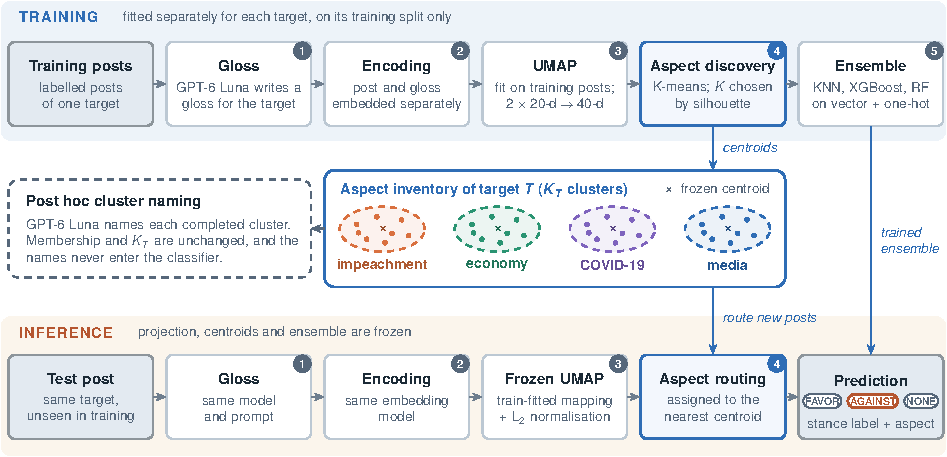
\includegraphics[width=\textwidth]{figures/workflow.pdf}
	\caption{Training and inference pipeline of \textit{AspectStance}. Training builds a target-specific aspect inventory and a stance ensemble; inference reuses the frozen UMAP mapping and centroids to route a new post before the soft-voting ensemble predicts its stance. One UMAP mapping, fitted on the training posts, reduces each view to 20 dimensions, and the two reduced views are concatenated into a 40-dimensional representation. \(L_2\) normalisation is applied only for clustering and routing, and routing assigns each new post to the nearest frozen centroid (Eq.~\eqref{eq:route}). The classifier receives the unnormalised 40-dimensional representation together with the one-hot encoding of the routed cluster, and the pipeline returns both a target-level stance label and the cluster index. The four cluster names shown are schematic.}
	\label{fig:overview}
\end{figure*}

\subsection{Target-conditioned text enrichment}\label{subsec42}

Tweets pack events, people, and judgements into a few words and leave much of the context to the reader. To make this context explicit, OpenAI's \textit{GPT-6 Luna} \cite{openai-gpt6-luna} writes a short explanation for each post--target pair, which we call the \emph{gloss}. The prompt (Figure~\ref{fig:prompt}) asks for 30--50 words that name the event, controversy, or aspect at issue and explain how the post relates to it. The model sometimes runs longer: two of the seven glosses reproduced in Section~\ref{sec:qualitative} have 59 words. The gloss thus gives a second, more explicit view of the post. We call the stage that produces it \emph{enrichment}; formally, for a post \(x\) and a target \(T\),
\begin{equation}\label{eq:enrich}
\tilde{x} = g(x, T),
\end{equation}
where \(g(\cdot,\cdot)\) denotes the language model under this prompt.

\begin{figure}[t]
	\centering
	\begin{tcolorbox}[colframe=snrule, colback=snbox, boxrule=0.6pt, arc=3pt, width=\linewidth, left=5pt, right=5pt, top=4pt, bottom=4pt]
		\footnotesize\ttfamily\raggedright\setlength{\parindent}{0pt}\setlength{\parskip}{0.25\baselineskip}\noindent
		Task: Explain how the tweet relates to the target. Identify the specific event, controversy, or aspect of the target it refers to. Briefly summarize that event or aspect and describe its connection to the tweet in 30-50 words. Do not quote the tweet; focus on interpretation and explanation.

		Tweet: "\ttlbrace input tweet here\ttrbrace" \\
		Target: "\ttlbrace input target here\ttrbrace"
	\end{tcolorbox}
	\caption{Enrichment prompt issued to OpenAI's \textit{GPT-6 Luna}. The post and its target are substituted into the braced fields, and the model returns a short gloss that relates the post to the target.}
	\label{fig:prompt}
\end{figure}

\subsection{Contextual representation}\label{subsec43}

The post and its gloss are encoded separately with OpenAI's \textit{text-embedding-3-large} \cite{openai-text-embedding-3-large}, denoted \(E(\cdot)\), which maps a text to a 3{,}072-dimensional vector. Keeping the two encodings separate means that the classifier always sees the post's own wording, not only the model's reading of it.

Each embedding is then reduced to 20 dimensions by a single UMAP mapping \(U\) \cite{mcinnes2018umap}, fitted for each target on the embeddings of the training posts only and then frozen. The same mapping also projects the gloss embeddings and, at inference, both embeddings of every test post. The representation of a post is therefore
\begin{equation}\label{eq:reduce}
v = [\,r;\, \tilde{r}\,] = \bigl[\,U(E(x));\, U(E(\tilde{x}))\,\bigr] \in \mathbb{R}^{40},
\end{equation}
where \([\cdot\,;\cdot]\) denotes concatenation and \(r\) and \(\tilde{r}\) are the reduced post and gloss vectors, which share one coordinate system. Sharing one mapping puts the two views in directly comparable coordinates. The price is that glosses are projected through a mapping fitted on posts, so \(\tilde{r}\) is an out-of-sample projection rather than a fitted embedding; Section~\ref{subsec73} returns to what this means for interpreting \(v\). No test post is used to fit the mapping.

For aspect assignment only, the representation is scaled to unit length,
\begin{equation}\label{eq:norm}
\hat{v} = \frac{v}{\lVert v \rVert_2},
\end{equation}
whereas the stance classifier receives the unnormalised \(v\).

\subsection{Target-specific aspect discovery}\label{subsec44}

Aspects are discovered by clustering the normalised training representations \(\hat{v}_i\) of each target (Eq.~\eqref{eq:norm}). For a given number of clusters \(K\), K-means \cite{lloyd1982least} assigns each vector to one of \(K\) clusters so as to minimise the squared Euclidean distance between every vector and the mean of its cluster. For unit-length vectors this distance equals \(2-2\cos\theta\), where \(\theta\) is the angle between them, so the clustering depends only on direction. The cluster means are not renormalised, which makes the method Euclidean K-means on normalised inputs rather than spherical K-means \cite{dhillon2001concept}.

We run K-means for every \(K\) from 2 to 30 and keep the partition with the highest mean cosine silhouette coefficient \cite{rousseeuw1987silhouettes}:
\begin{equation}\label{eq:silhouette}
K_T = \arg\max_{2 \le K \le 30}\; \frac{1}{N_T}\sum_{i=1}^{N_T} \frac{b_i - a_i}{\max(a_i,\, b_i)},
\end{equation}
where, in the \(K\)-cluster partition, \(a_i\) is the mean cosine distance from post \(i\) to the other members of its cluster and \(b_i\) is its mean cosine distance to the members of the nearest other cluster. Each term lies between \(-1\) and 1 and approaches 1 when a post is much closer to its own cluster than to any other. The sweep thus gives each target its own inventory size; Section~\ref{sec:inventories} reports the selected counts and scores.

The selected partition has \(K_T\) clusters, whose centroids \(\mu_{T,1}, \dots, \mu_{T,K_T}\) are frozen. Each training post \(x_i\) receives the index \(c_i\) of its cluster, which is its aspect in the sense of Eq.~\eqref{eq:aspects}; held-out posts are assigned by the routing rule of Eq.~\eqref{eq:route}. We use \emph{cluster} for the group of posts, \emph{aspect assignment} for its role as a classifier input, and \emph{aspect name} for its human-readable label. \(K_T\) should be read as a level of granularity chosen for one target in one representation, not as an estimate of how many facets the target really has. In the same spirit, a \emph{latent aspect} is simply a recurring region of this representation; it may reflect topic, rhetoric, or stance cues (Section~\ref{subsec73}).

\subsection{Post hoc cluster naming}\label{subsec45}

To make the clusters readable, we give \textit{GPT-6 Luna} the posts of each finished cluster and ask for a short, content-based description of its dominant theme (prompt in Appendix~\ref{secA11}); Section~\ref{sec:inventories} presents the resulting inventories. Naming only labels a fixed partition: the classifier sees the cluster index, while the tables and the qualitative analysis use the name of the same cluster.

\subsection{Aspect-conditioned stance model}\label{subsec46}

The classifier \(f_T\) of Eq.~\eqref{eq:predictor} is trained separately for each target. A post enters through its representation \(v\) and its aspect through a one-hot encoding, so the input of training post \(i\) is
\begin{equation}\label{eq:input}
z_i = \bigl[v_i; \operatorname{onehot}(c_i)\bigr] \in \mathbb{R}^{40 + K_T}.
\end{equation}
A one-hot encoding treats aspects as unordered categories; a single integer index would instead impose an arbitrary order on the distances computed by the nearest-neighbour member of the ensemble.

We implement \(f_T\) as an ensemble of three classifiers: k-nearest neighbours (KNN) \cite{cover1967nearest}, XGBoost \cite{chen2016xgboost}, and a random forest \cite{breiman2001random}, each trained on \(z_i\). The members are combined by \emph{soft} voting: each member \(m\) returns a distribution \(p_m(\cdot \mid z)\) over the label set, the three distributions are averaged with equal weight, and the label with the highest mean probability is predicted,
\begin{equation}\label{eq:vote}
\hat{y} = f_T(z) = \arg\max_{y \in \mathcal{Y}_T} \; \frac{1}{3}\sum_{m=1}^{3} p_m(y \mid z).
\end{equation}

\subsection{Inference: cluster routing and stance prediction}\label{subsec47}

Given a new post \(x\) for target \(T\), we compute its gloss, representation \(v\), and normalised vector \(\hat{v}\) exactly as in training (Eqs.~\eqref{eq:enrich}--\eqref{eq:norm}), using the \emph{frozen} UMAP mapping. The post is then assigned to the aspect whose training centroid is nearest:
\begin{equation}\label{eq:route}
h_T(x) = \arg\min_{k \in \{1,\dots,K_T\}} \bigl\lVert \hat{v} - \mu_{T,k} \bigr\rVert_2 .
\end{equation}
K-means forms its clusters by the same criterion (Section~\ref{subsec44}), so a test post is placed exactly as a training post in its neighbourhood would be; after convergence, the rule also reproduces the training assignments, \(c_i = h_T(x_i)\).

Finally, the ensemble predicts the stance from the unnormalised representation on which it was trained (Section~\ref{subsec46}) and the routed aspect:
\begin{equation}\label{eq:predict}
\hat{y} = f_T\bigl(\bigl[v;\, \operatorname{onehot}(h_T(x))\bigr]\bigr).
\end{equation}
Training and inference thus use the same two feature types. The stance label keeps the benchmark's target-level meaning, and the returned aspect index identifies the cluster used for conditioning, so each prediction can be inspected alongside the training posts of that cluster.

\begin{table*}[t]
	\caption{Stance-label distribution in the training and test splits for each target. P-Stance \cite{li2021p} has two stance labels; SemEval-2016 Task~6, Subtask~A \cite{mohammad2016semeval} adds a \textsc{none} class. ``Climate Change'' abbreviates the target ``Climate Change is a Real Concern''.}
	\label{tab:datasets}
	\centering
	\tablebodyfont
	\setlength{\tabcolsep}{0pt}
	\renewcommand{\arraystretch}{1.12}
	\begin{tabular*}{\textwidth}{@{\extracolsep{\fill}}lrrrrcrrrr@{}}
		\toprule
		& \multicolumn{4}{c}{\textbf{Training split}} && \multicolumn{4}{c}{\textbf{Test split}} \\
		\cmidrule{2-5}\cmidrule{7-10}
		\textbf{Target} & \textsc{favor} & \textsc{against} & \textsc{none} & Total && \textsc{favor} & \textsc{against} & \textsc{none} & Total \\
		\midrule
		\tabband{10}{\textsc{P-Stance}}
		Trump & 2,937 & 3,425 & -- & 6,362 && 361 & 435 & -- & 796 \\
		Biden & 2,552 & 3,254 & -- & 5,806 && 337 & 408 & -- & 745 \\
		Sanders & 2,858 & 2,198 & -- & 5,056 && 343 & 292 & -- & 635 \\
		\textit{All} & \textbf{8,347} & \textbf{8,877} & -- & \textbf{17,224} && \textbf{1,041} & \textbf{1,135} & -- & \textbf{2,176} \\
		\addlinespace[4pt]
		\tabband{10}{\textsc{SemEval-2016 Task~6, Subtask~A}}
		Atheism & 92 & 304 & 117 & 513 && 32 & 160 & 28 & 220 \\
		Climate Change & 212 & 15 & 168 & 395 && 123 & 11 & 35 & 169 \\
		Feminist Movement & 210 & 328 & 126 & 664 && 58 & 183 & 44 & 285 \\
		Hillary Clinton & 118 & 393 & 178 & 689 && 45 & 172 & 78 & 295 \\
		Legalization of Abortion & 121 & 355 & 177 & 653 && 46 & 189 & 45 & 280 \\
		\textit{All} & \textbf{753} & \textbf{1,395} & \textbf{766} & \textbf{2,914} && \textbf{304} & \textbf{715} & \textbf{230} & \textbf{1,249} \\
		\bottomrule
	\end{tabular*}
\end{table*}

\section{Experimental setup}\label{sec5}

\subsection{Datasets}\label{subsec51}
We evaluate \textit{AspectStance} on P-Stance \cite{li2021p} and on SemEval-2016 Task~6, Subtask~A \cite{mohammad2016semeval} (hereafter SemEval-2016). P-Stance covers three political figures with binary stance labels; Subtask~A covers five targets with three stance labels. Table~\ref{tab:datasets} reports, for each labelled set \(\mathcal{D}_T\) of Eq.~\eqref{eq:data}, the label distribution in its training and test splits. For P-Stance, models are fitted on the official training split and evaluated on the official test split; the validation split is not used for training, model selection, or evaluation. SemEval-2016 provides no separate validation split, so its official training data, including the 100 trial posts, and its official test split are used as released. In the tables and text, we abbreviate the SemEval-2016 target ``Climate Change is a Real Concern'' to ``Climate Change''; the full proposition still defines the stance target.


\subsection{Evaluation metric}\label{subsec52}
We report \(F1_{\mathrm{avg}}\), the official metric of SemEval-2016 Task~6 \cite{mohammad2016semeval}, which has also been adopted for P-Stance \cite{li2021p,li2023distilling}. For a given target, \(F1_{\mathrm{avg}}\) is the arithmetic mean of the F1 scores of the \textsc{favor} and \textsc{against} classes:
\begin{equation}\label{eq:f1avg}
F1_{\mathrm{avg}} = \frac{F1_{\textsc{favor}} + F1_{\textsc{against}}}{2}.
\end{equation}
The third SemEval-2016 class, \textsc{none}, is excluded from this average, following the official task definition. This class contains both genuinely neutral posts and posts from which no stance towards the target can be inferred. Because it is broader than ``neutral'', we retain the benchmark's own label throughout. Posts labelled \textsc{none} nevertheless remain part of the evaluation: predicting \textsc{favor} or \textsc{against} for a \textsc{none} post lowers the precision of the predicted class.

Two ways of aggregating over targets appear in the literature. The official Task~6 ranking pools predictions across all targets before computing the two class scores; the task paper calls this a micro-average across targets, \(F\text{-}\mathrm{micro}_T\). We instead use \(F\text{-}\mathrm{macro}_T = |\mathcal{T}|^{-1}\sum_{T\in\mathcal{T}} F1_{\mathrm{avg}}(T)\), where \(\mathcal{T}\) is the set of targets of a benchmark: \(F1_{\mathrm{avg}}\) is computed for each target and then averaged with equal weight over the five SemEval-2016 targets or the three P-Stance targets. P-Stance studies use the same convention \cite{li2023distilling}. Section~\ref{sec:published} flags published scores that use another metric or a different set of targets, so that they are not read as interchangeable with ours.

\subsection{Compared methods}\label{subsec53}
We compare \textit{AspectStance} with a cluster-feature ablation, a clustering-strategy control, and two prompting baselines, all run in this study.

\paragraph{Base Method.} This ablation trains the same per-target ensemble of KNN, XGBoost, and a random forest on the 40-dimensional vector \(v\) alone, without the one-hot cluster feature. In each run, the Base Method and \textit{AspectStance} share the glosses, the embeddings, the fitted UMAP mapping, and the equal-weight vote, so the cluster feature is the only design difference between the two arms. Each ensemble is still fitted from scratch on its own inputs, and library defaults that depend on the number of features, such as how many features the random forest considers at each split, therefore differ slightly between them. The comparison measures what cluster conditioning adds within this pipeline and under the settings of Section~\ref{subsec54}.

\paragraph{Random clustering.} The clustering-strategy control keeps the cluster feature but replaces the clustering method. For each target, the K-means partition of the training posts is replaced by a uniformly random assignment to \(K\) clusters. The centroids of these random clusters are computed on the \(L_2\)-normalised representation, and each test post is routed to the nearest of them by the rule of Eq.~\eqref{eq:route}. Every other component is unchanged: the data and splits, the glosses, the representation \(v\), the one-hot encoding, the ensemble, and the training and evaluation procedures. We vary \(K\) from 5 to 20, a range that contains every cluster count selected by the silhouette sweep (Section~\ref{sec:inventories}), and draw ten random assignments for each value of \(K\). Each of the resulting 160 configurations per target is run through the complete pipeline; the \(j\)-th random assignment for each \(K\) reuses the representation \(v\) of the \(j\)-th seeded run. For each target, we retain the highest test \(F1_{\mathrm{avg}}\) among these runs and then average the per-target maxima with the equal-target weighting of Section~\ref{subsec52}. Because the retained value is the best of 160 evaluations on the test split, whereas \textit{AspectStance} is represented by its ten-seed mean, this selection favours the random-clustering control.

\paragraph{Zero-shot prompting.} We prompt \textit{GPT-6 Luna} directly to predict the stance of each test post towards its target, without any training examples (Appendix~\ref{secA12}).

\paragraph{Retrieval-augmented few-shot prompting.} This baseline adds labelled examples, retrieved from the training split of the same target, to the prompt before asking \textit{GPT-6 Luna} for the stance of the test post (Appendix~\ref{secA13}). Retrieval is balanced across labels: for each test post and \emph{each} label class, we take the five training posts of that class whose \textit{text-embedding-3-large} embeddings have the highest cosine similarity to the embedding of the test post. This yields 15 examples for SemEval-2016 and 10 for P-Stance, which has no \textsc{none} class. Every label is represented equally, whatever the label distribution of the target's training split, and no example can come from another target or from the test split. Balanced retrieval guarantees that each label is illustrated, but it hides the class prior and may push the model towards minority labels such as \textsc{against} on Climate Change.

\paragraph{Published systems.} Section~\ref{sec:published} reports selected results from the literature. Each score is reported with its original setting, since evaluation protocols and target coverage vary across studies.

\subsection{Implementation details}\label{subsec54}
As described in Section~\ref{sec4}, enrichment uses OpenAI \textit{GPT-6 Luna} with the prompt in Figure~\ref{fig:prompt}, and both views are encoded with \textit{text-embedding-3-large} (3{,}072 dimensions per input). UMAP is run with \texttt{n\_components}~=~20, \texttt{n\_neighbors}~=~15, \texttt{min\_dist}~=~0.1, and the cosine distance metric. The output dimensionality and the metric depart from the library defaults. The cosine metric only determines how UMAP builds its neighbourhood graph from the input embeddings; the output space is Euclidean with an arbitrary origin, so normalising the output vectors (Eq.~\eqref{eq:norm}) is a separate design choice. These settings matter because the reduced space, and with it both the silhouette sweep and the induced partition, depends on them. All remaining K-means and classifier settings are the scikit-learn and XGBoost library defaults. Every \textit{GPT-6 Luna} call (API model \texttt{gpt-6-luna}) uses the \texttt{medium} reasoning-effort setting. All other parameters keep the provider's defaults.

Every score reported for \textit{AspectStance} and the Base Method is the mean of ten runs that differ only in the random seed. The glosses and their embeddings are generated once and reused across runs, whereas UMAP, the cluster-count sweep, clustering, and all three ensemble members are refitted in every run. With default settings, KNN and XGBoost are deterministic given their input, so within the supervised stage only the random forest draws on the seed. The ten runs thus sample the randomness of both the clustering and the classification stage. The two prompting baselines have no seed of their own, and repeated calls to the language model need not return identical outputs, so we pass the test split through each baseline ten times and report the mean and standard deviation over these passes in Section~\ref{sec:main}. A response that contains no valid label is counted as an error. Means are reported to one decimal place, the precision at which they were recorded, and across-run standard deviations to two.

All design choices described in Section~\ref{sec4} were fixed before any test post was scored, including the reduced dimensionality, the sweep range, the restriction of \(L_2\) normalisation to the clustering branch, and the equal voting weights. Test labels played no part in selecting \textit{AspectStance} or the Base Method. The only selection on the test split is the per-target maximum of the random-clustering control, which favours that control (Section~\ref{subsec53}). Appendix~\ref{secA1} gives the three remaining prompts and the retrieval rule for the few-shot baseline.

\section{Results}\label{sec6}

\begin{figure*}[t]
	\centering
	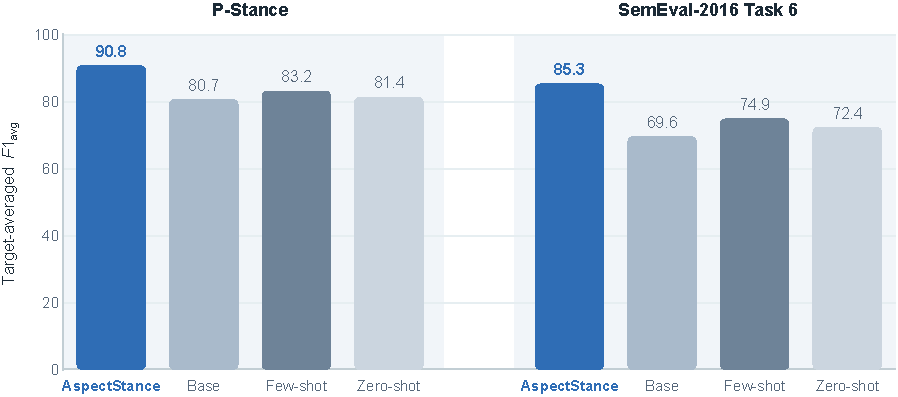
\includegraphics[width=\textwidth]{figures/main_results.pdf}
	\caption{Target-averaged \textsc{favor}/\textsc{against} F1 (\(F\text{-}\mathrm{macro}_T\)) on each benchmark for \textit{AspectStance}, the Base Method (the same ensemble without the cluster feature), and the retrieval-augmented few-shot and zero-shot \textit{GPT-6 Luna} baselines (Section~\ref{subsec53}). Bars are means over ten runs: seeded refits for \textit{AspectStance} and the Base Method, and passes over the test split for the prompting baselines. Across-run standard deviations are reported in Table~\ref{tab:pertarget} and Section~\ref{sec:main}.}
	\label{fig:results}
\end{figure*}

We first evaluate the cluster-feature ablation across targets and seeds (RQ1 and RQ2) and the clustering-strategy control (RQ3), and then examine the induced inventories (RQ4). The last two subsections compare the results with published systems and analyse representative glosses.

\subsection{Main results}\label{sec:main}

Figure~\ref{fig:results} summarises the main comparison. \textit{AspectStance} reaches a target-averaged \(F1_{\mathrm{avg}}\) (\(F\text{-}\mathrm{macro}_T\); Section~\ref{subsec52}) of 90.8 on P-Stance and 85.3 on SemEval-2016, ahead of the Base Method and both prompting baselines.

The Base Method scores 80.7 on P-Stance and 69.6 on SemEval-2016, so the cluster feature adds 10.1 and 15.7 F1 points, respectively. Because the one-hot cluster feature is the only design difference between the two arms (Section~\ref{subsec53}), these margins measure the benefit of exposing that feature to the ensemble. Section~\ref{subsec71} discusses where this benefit comes from.

\begin{table}[t]
	\caption{Per-target \(F1_{\mathrm{avg}}\) on the official test splits for \textit{AspectStance} and the matched Base Method (no cluster feature). Entries are means over ten seeded runs with across-run standard deviations; \(\Delta\) is \textit{AspectStance} minus Base, in F1 points. \textit{Target average} rows give the equal-weight mean over targets (\(F\text{-}\mathrm{macro}_T\), Section~\ref{subsec52}). Within each benchmark, targets are listed in descending order of \textit{AspectStance} score.}
	\label{tab:pertarget}
	\centering
	\tablebodyfont
	\setlength{\tabcolsep}{1pt}
	\renewcommand{\arraystretch}{1.15}
	\begin{tabular*}{\linewidth}{@{\extracolsep{\fill}}lccc@{}}
		\toprule
		\textbf{Target} & \textbf{\textit{AspectStance}} & \textbf{Base} & $\boldsymbol{\Delta}$ \\
		\midrule
		\tabband{4}{\textsc{P-Stance}}
		Trump                      & 91.6\,\sd{0.35} & 82.1\,\sd{0.33} & $\phantom{0}{+}9.5$ \\
		Biden                      & 90.9\,\sd{0.33} & 80.7\,\sd{0.15} & $+10.2$ \\
		Sanders                    & 89.9\,\sd{0.28} & 79.3\,\sd{0.44} & $+10.6$ \\
		\cmidrule{1-4}
		\textit{Target average} & \textbf{90.8}\,\sd{0.29} & \textbf{80.7}\,\sd{0.21} & $\mathbf{+10.1}$ \\
		\addlinespace[6pt]
		\tabband{4}{\textsc{SemEval-2016 Task~6}}
		Atheism                    & 88.9\,\sd{0.15} & 74.2\,\sd{0.18} & $+14.7$ \\
		Legalization of Abortion   & 87.4\,\sd{0.39} & 71.3\,\sd{0.36} & $+16.1$ \\
		Hillary Clinton            & 85.9\,\sd{0.35} & 69.8\,\sd{0.33} & $+16.1$ \\
		Feminist Movement          & 84.2\,\sd{0.45} & 67.9\,\sd{0.51} & $+16.3$ \\
		Climate Change             & 80.2\,\sd{0.51} & 64.8\,\sd{0.55} & $+15.4$ \\
		\cmidrule{1-4}
		\textit{Target average} & \textbf{85.3}\,\sd{0.34} & \textbf{69.6}\,\sd{0.31} & $\mathbf{+15.7}$ \\
		\bottomrule
	\end{tabular*}
\end{table}

Table~\ref{tab:pertarget} breaks the aggregate gains down by target. The gain is positive on every target, ranging from 9.5 to 10.6 points on P-Stance and from 14.7 to 16.3 points on SemEval-2016, a spread of only 1.1 and 1.6 points within the two benchmarks. No across-run standard deviation exceeds 0.55, so on every target the margin between the two systems is far larger than the run-to-run spread.

The benchmarks also differ in the spread of absolute scores. Under \textit{AspectStance}, the three P-Stance targets lie within 1.7 points of one another, from 89.9 to 91.6, whereas the five SemEval-2016 targets span 8.7 points, from 80.2 to 88.9. Climate Change is the most difficult target for both systems: its test split contains only 11 \textsc{against} posts, compared with 123 \textsc{favor} posts, so the \textsc{against} term in Eq.~\eqref{eq:f1avg} is especially sensitive to individual predictions. Feminist Movement, the second most difficult target, also has the least differentiated inventory, with 496 of its 664 training posts in its largest cluster.

Zero-shot \textit{GPT-6 Luna} scores 81.4\,\(\pm\)\,0.25 on P-Stance and 72.4\,\(\pm\)\,0.29 on SemEval-2016, and retrieval-augmented few-shot prompting raises these scores to 83.2\,\(\pm\)\,0.21 and 74.9\,\(\pm\)\,0.19; \textit{AspectStance} exceeds the stronger, few-shot baseline by 7.6 and 10.4 points. These comparisons, however, span different supervision regimes: the zero-shot prompt receives only the test post and its target, the few-shot prompt adds retrieved labelled examples, and \textit{AspectStance} trains a classifier for each target. Only the Base Method and the random-clustering control of Section~\ref{sec:random} are controlled ablations of cluster conditioning.

\subsection{Clustering-strategy control}\label{sec:random}

The Base Method shows that the cluster feature matters. The random-clustering control asks whether it also matters how the clusters are formed (RQ3). Table~\ref{tab:random} sets both controls beside \textit{AspectStance}. With random clustering in place of K-means and the rest of the pipeline unchanged, the target-averaged score falls from 90.8 to 75.7 on P-Stance and from 85.3 to 74.1 on SemEval-2016, losses of 15.1 and 11.2 points. This comparison favours the control, because each random entry is the best of 160 complete runs for its target, selected on the test split, whereas \textit{AspectStance} enters with its ten-seed mean. Even under this selection, random clustering stays more than 11 points below the induced partition on both benchmarks. This answers RQ3: the gain in Section~\ref{sec:main} depends on how the clusters are formed, not merely on having a cluster feature.

\begin{table}[t]
	\caption{Clustering-strategy control: target-averaged \(F1_{\mathrm{avg}}\) (\(F\text{-}\mathrm{macro}_T\)). \textit{AspectStance} and the Base Method are ten-seed means (Table~\ref{tab:pertarget}). The random-clustering row replaces K-means with random clustering, keeps every other component fixed, and reports the equal-target mean of each target's best test score over 160 complete runs (\(K=5,\ldots,20\), ten random assignments per \(K\); Section~\ref{subsec53}). \(\Delta\) is the difference from \textit{AspectStance}.}
	\label{tab:random}
	\centering
	\tablebodyfont
	\setlength{\tabcolsep}{2pt}
	\renewcommand{\arraystretch}{1.15}
	\begin{tabular*}{\linewidth}{@{\extracolsep{\fill}}lcccc@{}}
		\toprule
		& \multicolumn{2}{c}{\textbf{P-Stance}} & \multicolumn{2}{c}{\textbf{SemEval-2016}} \\
		\cmidrule(lr){2-3}\cmidrule(l){4-5}
		\textbf{Clustering} & \(F1_{\mathrm{avg}}\) & \(\Delta\) & \(F1_{\mathrm{avg}}\) & \(\Delta\) \\
		\midrule
		K-means (\textit{AspectStance}) & \textbf{90.8} & -- & \textbf{85.3} & -- \\
		Random clustering & 75.7 & \(-15.1\) & 74.1 & \(-11.2\) \\
		None (Base Method) & 80.7 & \(-10.1\) & 69.6 & \(-15.7\) \\
		\bottomrule
	\end{tabular*}
\end{table}

\begin{table*}[t]
	\caption{Target-specific latent aspect inventories for P-Stance, from one of the ten runs. Each shaded band gives the target, its selected cluster count $K$, and the cosine silhouette coefficient (Sil.) of the selected partition, computed on the $L_2$-normalised 40-dimensional training representation; $n$ is the number of training posts assigned to each cluster, and the share column gives that number as a percentage of the target's training posts. Clusters are listed in descending order of size; names were generated post hoc by \textit{GPT-6 Luna} (Section~\ref{subsec45}).}
	\label{tab:aspects_pstance}
	\centering
	\tablebodyfont
	\setlength{\tabcolsep}{4pt}
	\renewcommand{\arraystretch}{1.1}
	\begin{tabular}{@{}L{0.58\textwidth}r@{\hspace{12pt}}r@{\hspace{5pt}}p{1.75cm}@{}}
		\toprule
		\textbf{Generated aspect name} & $\boldsymbol{n}$ & \multicolumn{2}{c}{\textbf{Share (\%)}} \\
		\midrule
		\aspecthead{Trump}{16}{0.91}
		Direct messages to Trump / POTUS (addressing him directly) & 1,160 & 18.2 & \sbar{18.2} \\
		Sparse-content and cross-cutting mentions & 936 & 14.7 & \sbar{14.7} \\
		Elections, voting, and campaign dynamics & 850 & 13.4 & \sbar{13.4} \\
		Partisan conflict and congressional politics (Dems vs GOP) & 732 & 11.5 & \sbar{11.5} \\
		Investigations, corruption, and legal scandals & 470 & 7.4 & \sbar{7.4} \\
		Impeachment and accountability (impeachment, resign, jail, 25th) & 399 & 6.3 & \sbar{6.3} \\
		COVID-19 / coronavirus response and public health debate & 310 & 4.9 & \sbar{4.9} \\
		Pro-Trump praise, MAGA slogans, and rally enthusiasm & 267 & 4.2 & \sbar{4.2} \\
		Media, ``fake news'', and conflicts with platforms & 249 & 3.9 & \sbar{3.9} \\
		Anti-Trump character attacks, ridicule, and insults & 231 & 3.6 & \sbar{3.6} \\
		Economy, jobs, markets, taxes, and trade & 197 & 3.1 & \sbar{3.1} \\
		Immigration, border, asylum, and the wall & 139 & 2.2 & \sbar{2.2} \\
		Foreign policy and national security & 139 & 2.2 & \sbar{2.2} \\
		Democracy, constitution, rule-of-law, and authoritarianism framing & 112 & 1.8 & \sbar{1.8} \\
		Race, policing, protests, and civil unrest & 111 & 1.7 & \sbar{1.7} \\
		Conspiracy, QAnon, and ``deep state'' narratives & 60 & 0.9 & \sbar{0.9} \\
		\addlinespace[3pt]
		\aspecthead{Biden}{12}{0.89}
		Broad political commentary and cross-cutting mentions & 1,175 & 20.2 & \sbar{20.2} \\
		Scandals, allegations, and controversy narratives & 1,051 & 18.1 & \sbar{18.1} \\
		Obama-era/VP legacy and major Democratic relationships & 723 & 12.5 & \sbar{12.5} \\
		Campaign updates (events, appearances, media coverage) & 588 & 10.1 & \sbar{10.1} \\
		Debates and comparisons with other Democratic candidates & 447 & 7.7 & \sbar{7.7} \\
		Policy positions and issue proposals & 377 & 6.5 & \sbar{6.5} \\
		General praise/support for Biden's leadership and character & 329 & 5.7 & \sbar{5.7} \\
		General criticism/attacks on Biden (non-scandal) & 286 & 4.9 & \sbar{4.9} \\
		Election results, polls, primaries, and delegate math & 283 & 4.9 & \sbar{4.9} \\
		Fundraising, volunteering, and voter mobilization & 258 & 4.4 & \sbar{4.4} \\
		Trump matchup and anti-Trump / anti-GOP framing & 189 & 3.3 & \sbar{3.3} \\
		Personal anecdotes, humor, and pop-culture side chatter & 100 & 1.7 & \sbar{1.7} \\
		\addlinespace[3pt]
		\aspecthead{Sanders}{9}{0.93}
		Polls, primaries, elections, and campaign developments & 995 & 19.7 & \sbar{19.7} \\
		Neutral commentary, links, quotes, and miscellaneous mentions & 975 & 19.3 & \sbar{19.3} \\
		DNC/establishment and media-bias or ``rigging'' narratives & 845 & 16.7 & \sbar{16.7} \\
		Comparisons with other Democrats and debate-focused discussion & 777 & 15.4 & \sbar{15.4} \\
		Policy and issue advocacy & 472 & 9.3 & \sbar{9.3} \\
		Anti-Bernie criticism and attacks & 472 & 9.3 & \sbar{9.3} \\
		Pro-Bernie support, movement slogans, and encouragement & 256 & 5.1 & \sbar{5.1} \\
		Fundraising, donations, and volunteer organizing & 210 & 4.2 & \sbar{4.2} \\
		GOP/Republican contrast and partisan framing & 54 & 1.1 & \sbar{1.1} \\
		\bottomrule
	\end{tabular}
\end{table*}

\begin{table*}[t]
	\caption{Target-specific latent aspect inventories for SemEval-2016 Task~6, Subtask~A, from one of the ten runs. Bands, $K$, Sil., $n$, the share column and the ordering of clusters are as in Table~\ref{tab:aspects_pstance}; names were generated post hoc by \textit{GPT-6 Luna} (Section~\ref{subsec45}).}
	\label{tab:aspects_semeval}
	\centering
	\tablebodyfont
	\setlength{\tabcolsep}{4pt}
	\renewcommand{\arraystretch}{1.1}
	\begin{tabular}{@{}L{0.58\textwidth}r@{\hspace{12pt}}r@{\hspace{5pt}}p{1.75cm}@{}}
		\toprule
		\textbf{Generated aspect name} & $\boldsymbol{n}$ & \multicolumn{2}{c}{\textbf{Share (\%)}} \\
		\midrule
		\aspecthead{Atheism}{5}{0.94}
		Debates, skepticism, humor, and miscellaneous commentary & 198 & 38.6 & \sbar{38.6} \\
		Faith-based encouragement and spiritual reflections & 135 & 26.3 & \sbar{26.3} \\
		Prayer, worship, and devotional praise & 75 & 14.6 & \sbar{14.6} \\
		Scripture citations and verse quotations & 59 & 11.5 & \sbar{11.5} \\
		Religion in social/political debates (equality, law, public life) & 46 & 9.0 & \sbar{9.0} \\
		\addlinespace[3pt]
		\aspecthead{Climate Change}{5}{0.87}
		Broad climate-change discussion and cross-cutting themes & 233 & 59.0 & \sbar{59.0} \\
		Everyday weather anecdotes and seasonal oddities & 54 & 13.7 & \sbar{13.7} \\
		Politics, policy, and politicized arguments (incl.\ denial/hoax claims) & 44 & 11.1 & \sbar{11.1} \\
		Personal action, awareness, and solutions (sustainability + energy) & 34 & 8.6 & \sbar{8.6} \\
		Scientific evidence, measurements, and physical impacts & 30 & 7.6 & \sbar{7.6} \\
		\addlinespace[3pt]
		\aspecthead{Feminist Movement}{5}{0.85}
		General discussions of feminism, gender roles, and equality debates & 496 & 74.7 & \sbar{74.7} \\
		Gamergate and online gaming culture disputes & 61 & 9.2 & \sbar{9.2} \\
		Sexism, misogyny, harassment, and violence against women & 38 & 5.7 & \sbar{5.7} \\
		Pro-feminism advocacy, empowerment, and equality messaging & 37 & 5.6 & \sbar{5.6} \\
		Backlash, anti-feminism, and men's-rights framing & 32 & 4.8 & \sbar{4.8} \\
		\addlinespace[3pt]
		\aspecthead{Hillary Clinton}{6}{0.89}
		General mentions and miscellaneous commentary & 387 & 56.2 & \sbar{56.2} \\
		Email/Benghazi/ethics scandals and corruption narratives & 73 & 10.6 & \sbar{10.6} \\
		Campaign, elections, polling, and voting talk & 71 & 10.3 & \sbar{10.3} \\
		Comparisons with other politicians and party politics & 57 & 8.3 & \sbar{8.3} \\
		Support, admiration, and pro-Hillary enthusiasm & 52 & 7.5 & \sbar{7.5} \\
		Hostile attacks, memes, and criminality claims (``lock her up'') & 49 & 7.1 & \sbar{7.1} \\
		\addlinespace[3pt]
		\aspecthead{Legalization of Abortion}{5}{0.92}
		Pro-life moral framing and general abortion debates & 422 & 64.6 & \sbar{64.6} \\
		Courts, laws, and legislation (SCOTUS, Roe v.\ Wade, bills) & 81 & 12.4 & \sbar{12.4} \\
		Healthcare context: clinics, contraception, and exception cases & 56 & 8.6 & \sbar{8.6} \\
		Religion-based arguments and prayerful appeals & 49 & 7.5 & \sbar{7.5} \\
		Pro-choice autonomy and women's rights framing & 45 & 6.9 & \sbar{6.9} \\
		\bottomrule
	\end{tabular}
\end{table*}

The two benchmarks differ in where the random-clustering control falls relative to the Base Method. On P-Stance, the best random configurations score 5.0 points below the Base Method, which receives no cluster feature at all, whereas on SemEval-2016 they lie 4.5 points above it. A random partition is not a neutral addition. The ensemble responds strongly to the one-hot cluster feature, and whether that response helps depends on the clustering behind it. Under random assignment, moreover, the routing rule of Eq.~\eqref{eq:route} no longer reproduces the training assignments in general: training posts keep their random cluster index, whereas each test post receives the index of its nearest random centroid. The control therefore changes both the partition and the agreement between training and test assignments, and it does not separate these two effects. The 4.5-point margin on SemEval-2016 should also be read with the selection in mind, since with 169 to 295 test posts per target the maximum of 160 evaluations is an optimistic estimate.

Two invariance checks, relabelling the cluster indices consistently in training and test and permuting the order of the one-hot columns, left the scores essentially unchanged, so the results do not depend on the arbitrary numbering of the clusters.

\subsection{Induced aspect inventories}\label{sec:inventories}

Tables~\ref{tab:aspects_pstance} and~\ref{tab:aspects_semeval} report the selected cluster counts, cosine silhouette coefficients, generated names, and cluster sizes. The inventories contain 9 to 16 clusters per P-Stance target and 5 or 6 per SemEval-2016 target. The reported silhouette values, computed on the training posts in the reduced representation used for selection, range from 0.85 to 0.94. They determine the size of each inventory, and Section~\ref{subsec73} discusses how to interpret them. The sweep selected the same \(K_T\) for each target in all ten runs, so the inventory size is stable under reseeding even though UMAP and K-means are refitted in every run.
The generated names and cluster sizes in the two tables are taken from one of these runs.

\begin{table*}[t]
	\caption{Selected published results on each benchmark (0--100 scale), with \textit{AspectStance} first and the other systems in descending order of score. Scores are target-averaged \(F1_{\mathrm{avg}}\) as reported by each source, with two exceptions: the topic-guided transformer reports macro-F1, and MPRF reports F-macro, which on the binary P-Stance coincides with \(F1_{\mathrm{avg}}\) for each target. On SemEval-2016, KASD evaluates three targets and MPVStance six; for MPVStance we report the mean of its six per-target scores (Section~\ref{sec:published}). BERTweet scores are those reported by KASD \cite{li2023stance}. Published scores are rounded to one decimal place.}
	\label{tab:published}
	\centering
	\setlength{\tabcolsep}{6pt}
	\renewcommand{\arraystretch}{1.18}
	\tablebodyfont
	\begin{tabularx}{\textwidth}{@{}>{\hsize=0.85\hsize}Y >{\hsize=1.15\hsize}Y r@{}}
		\toprule
		\textbf{Method} & \textbf{Approach} & \textbf{Score} \\
		\midrule
		\tabband{3}{\textsc{P-Stance}}
		\textit{AspectStance} (ours) & Per-target ensemble with an LLM gloss & \textbf{90.8} \\
		\addlinespace[2pt]
		MPRF \cite{zhang2025mprf} & Multi-path LLM reasoning & 88.4 \\
		\addlinespace[2pt]
		KASD-BERT \cite{li2023stance} & Encoder with LLM-processed knowledge & 83.8 \\
		\addlinespace[2pt]
		KASD-ChatGPT \cite{li2023stance} & LLM with retrieved knowledge & 83.2 \\
		\addlinespace[2pt]
		BERTweet \cite{nguyen2020bertweet} & Fine-tuned encoder & 82.1 \\
		\addlinespace[2pt]
		CKD \cite{li2023distilling} & Calibrated distillation & 82.0 \\
		\addlinespace[6pt]
		\tabband{3}{\textsc{SemEval-2016 Task~6}}
		\textit{AspectStance} (ours) & Per-target ensemble with an LLM gloss & \textbf{85.3} \\
		\addlinespace[2pt]
		MPVStance \cite{zhang2025mpvstance} & Multi-perspective LLM verification & 82.2 \\
		\addlinespace[2pt]
		Topic-guided transformer \cite{muthusami2025interpretable} & Topic features with RoBERTa & 78.4 \\
		\addlinespace[2pt]
		KASD-BERT \cite{li2023stance} & Encoder with LLM-processed knowledge & 73.4 \\
		\addlinespace[2pt]
		KASD-ChatGPT \cite{li2023stance} & LLM with retrieved knowledge & 71.5 \\
		\addlinespace[2pt]
		BERTweet \cite{nguyen2020bertweet} & Fine-tuned encoder & 63.6 \\
		\bottomrule
	\end{tabularx}
\end{table*}

Cluster sizes show that thematic concentration differs across targets. On SemEval-2016, the largest cluster holds between 39\% (Atheism) and 75\% (Feminist Movement) of a target's training posts, and its generated name often describes broad, recurring discourse that cuts across narrower topics.

Turning to RQ4, most clusters correspond to a recognisable subtopic of their target: impeachment, COVID-19, immigration, and the economy for Trump; fundraising, polls, and debates for Biden and Sanders; Gamergate for Feminist Movement; and courts and legislation for Legalization of Abortion. The inventories also contain two other kinds of cluster. In five of the eight targets, the largest cluster is named as broad, general, or miscellaneous; in the other three it is a substantive theme (polls and primaries for Sanders, pro-life moral framing for Legalization of Abortion) or, for Trump, a form of address: direct messages to the president. In addition, 12 of the 63 names describe a pro- or anti-target orientation (for example, ``Pro-Trump praise'' and ``Anti-Trump character attacks''). The discovered aspects are mostly subtopics, although some clusters mix topic with rhetoric or stance cues (Section~\ref{subsec73}).

\subsection{Comparison with prior work}\label{sec:published}

Table~\ref{tab:published} sets our results beside those of selected published systems on the same benchmarks, recording for each the approach and the metric reported by the source. Our SemEval-2016 result averages over the five Subtask~A targets. Some LLM evaluations, including that of MPVStance, add Donald Trump, the target of Subtask~B, as a sixth target, and the official ranking instead pools predictions across targets.

\begin{table*}[p]
	\caption{Illustrative P-Stance training posts and their glosses. The posts are lightly paraphrased to hinder re-identification of their authors; the glosses are reproduced verbatim.}
	\label{tab:examples_pstance}
	\centering
	\tablebodyfont\hyphenpenalty=10000\exhyphenpenalty=10000
	\setlength{\tabcolsep}{5pt}
	\renewcommand{\arraystretch}{1.12}
	\begin{tabular}{@{}L{0.295\textwidth}L{0.085\textwidth}L{0.545\textwidth}@{}}
		\toprule
		\textbf{Post} & \textbf{Target} & \textbf{Gloss} \\
		\midrule
		\#PRESIDENT TRUMP thanks Damian Paletta for telling federal workers that First Bank of Oklahoma will keep their paychecks coming despite Democrats who mislead voters! Call the bank for paycheck support. We will stop the Dems from helping crime! & Trump & The tweet positions former President Trump as a champion of government workers, praising journalist Damian Paletta for highlighting that First Bank of Oklahoma ensured uninterrupted paychecks despite alleged Democratic failures. It frames Democrats as deceptive and suggests Trump's leadership actively defends workers and combats crime, reinforcing his image as a protector of everyday Americans and critic of political opponents. \\
		\addlinespace[3pt]
		The JRE episode with @BernieSanders has passed 4 million YouTube views and is still trending at \#1. This is only the beginning! & Sanders & The tweet celebrates the success of Bernie Sanders' appearance on the Joe Rogan Experience, highlighting its viral impact with 4 million views and a top trending position on YouTube. It frames Sanders as a figure generating widespread public interest, signaling growing momentum around his ideas, while conveying optimism that this exposure is only the beginning of his expanding reach. \\
		\bottomrule
	\end{tabular}
\end{table*}

\begin{table*}[p]
	\caption{Illustrative SemEval-2016 Task~6 training posts and their glosses, presented as in Table~\ref{tab:examples_pstance} (posts lightly paraphrased, glosses verbatim).}
	\label{tab:examples_semeval}
	\centering
	\tablebodyfont\hyphenpenalty=10000\exhyphenpenalty=10000
	\setlength{\tabcolsep}{5pt}
	\renewcommand{\arraystretch}{1.12}
	\begin{tabular}{@{}L{0.295\textwidth}L{0.105\textwidth}L{0.525\textwidth}@{}}
		\toprule
		\textbf{Post} & \textbf{Target} & \textbf{Gloss} \\
		\midrule
		Break free from every circle of limitation and affliction in the name of Jesus. \#solutionnight \#goodthing \#SemST & Atheism & The tweet contrasts with atheism by invoking faith in Jesus as a solution to personal struggles. It references the belief in spiritual deliverance from limitations or afflictions, highlighting a worldview centered on divine intervention, which directly opposes atheism's rejection of religious or supernatural explanations for life's challenges. \\
		\addlinespace[3pt]
		Did u know \#SCOTUS will decide whether \#Coal plants may keep \#Emitting unlimited \#Mercury into our atmosphere? \#POTUS \#Gop \#Justices \#SemST & Climate Change & The tweet refers to a Supreme Court case evaluating whether coal-fired power plants can continue releasing mercury into the atmosphere without stricter limits. This connects to climate change because mercury emissions contribute to pollution and environmental degradation, highlighting ongoing legal and political debates over regulating harmful industrial emissions. \\
		\addlinespace[3pt]
		Obsessed with becoming a woman who is comfortable in her own skin (Sandra Cisneros). \#latinx \#woc \#SemST & Feminist Movement & The tweet reflects the feminist movement's emphasis on self-acceptance, empowerment, and body autonomy for women. By expressing a desire to be comfortable in her skin, it connects to the movement's advocacy for challenging societal beauty standards and embracing women's diverse identities, particularly highlighting intersections of race and culture. \\
		\addlinespace[3pt]
		@CBSThisMorning Missing and incomplete emails? Who would have guessed? I'M ABOVE THE LAW, the rest of you are peons! JUST TRUST ME! \#SemST & Hillary Clinton & The tweet references the controversy over Hillary Clinton's use of a private email server during her tenure as Secretary of State. It alludes to missing or incomplete emails and perceived arrogance or disregard for rules, highlighting public criticism that she acted above legal and ethical standards. \\
		\addlinespace[3pt]
		There is a clear inverse correlation between a woman's right to choose and crime rates \#womensrights \#SemST & Legalization of Abortion & The tweet suggests that access to abortion may influence societal outcomes, implying that regions with greater reproductive rights experience lower crime rates. This references research linking the legalization of abortion to reduced future crime, as unwanted births, often associated with economic hardship or instability, can contribute to higher crime. \\
		\bottomrule
	\end{tabular}
\end{table*}

On P-Stance, the in-target systems reported by KASD use the same equal-target \textsc{favor}/\textsc{against} aggregation as we do. \textit{AspectStance} scores about seven points above KASD-BERT (90.8 versus 83.8) and about nine points above fine-tuned BERTweet \cite{nguyen2020bertweet} (82.1, as reported by KASD). MPRF reports an F-macro of 88.4 on P-Stance, which for this binary benchmark coincides with \(F1_{\mathrm{avg}}\) on each target; it uses multi-path LLM reasoning with Mistral-7B-Instruct rather than a classifier trained for each target. On the three SemEval-2016 targets for which KASD reports in-target results (Hillary Clinton, Feminist Movement, and Legalization of Abortion), \textit{AspectStance} averages 85.8, compared with 73.4 for KASD-BERT, 71.5 for KASD-ChatGPT, and 63.6 for BERTweet. The KASD systems and BERTweet share the metric and the targets but differ in encoder and training protocol. Like \textit{AspectStance}, KASD enriches each post with LLM-generated text.

On both benchmarks, \textit{AspectStance} has the highest score in Table~\ref{tab:published}, but no row is a controlled comparison: the systems differ in approach, in the number of targets, and in whether a language model is consulted at inference. The evidence for cluster conditioning therefore rests on the controlled ablations in Tables~\ref{tab:pertarget} and~\ref{tab:random} rather than on cross-paper comparison.

\subsection{Qualitative analysis}\label{sec:qualitative}

Tables~\ref{tab:examples_pstance} and~\ref{tab:examples_semeval} pair training posts with their glosses. In several cases, the gloss makes an allusion or abbreviation explicit before the text is embedded: it links a remark about Hillary Clinton's missing emails to the private-server controversy, identifies the claim behind the abortion--crime statement, and expands ``JRE'' to \textit{The Joe Rogan Experience}.

The same examples show that the gloss goes beyond paraphrase and interprets the post. It reads a religious appeal as opposition to Atheism and connects mercury regulation to Climate Change through environmental policy, a topical leap that the post itself does not make. Because the post is encoded in a separate branch, the added context supplements the post's wording without replacing it, although this supplement is not stance-neutral (Section~\ref{subsec73}).

\section{Discussion}\label{sec7}

\subsection{Interpreting the gain from cluster conditioning}\label{subsec71}

Taken together, the controls answer RQ1--RQ3. The cluster feature improves an otherwise identical ensemble (RQ1). The gain holds on every target and is more than an order of magnitude larger than the run-to-run spread, so no single target or favourable seed carries it (RQ2). And it shrinks sharply, or turns negative, when the clusters are random, even though random clustering is given the best of 160 configurations per target (RQ3). What helps, in other words, is the induced partition, not the extra feature as such.

Why should a deterministic function of \(v\) help a classifier that already receives \(v\)? The cluster feature adds no new observation. It changes how existing information is presented to the classifier, and we see three complementary ways in which this can help.

\emph{Discretisation as an inductive bias.} The one-hot block exposes a partition as a categorical feature on which the tree-based members can split directly, and it alters the distances that the KNN member computes: two posts in different clusters are separated by an additional 2 in squared Euclidean distance. Finite-sample learners with default settings would otherwise have to reconstruct the partition from continuous coordinates. The random-clustering control shows that this channel can help or hurt depending on the partition it carries: with random clusters, the P-Stance score even falls below that of the Base Method.

\emph{Coherent groups.} K-means places similar posts in the same cluster, so each cluster marks a coherent region of the reduced space, whereas a random cluster mixes posts from all regions. The gap between K-means and random clustering is consistent with this effect, although the control does not separate coherence from other properties of the partition, such as its cluster sizes.

\emph{Aspect-specific stance regularities.} Most clusters correspond to subtopics of the target and so delimit regions of discourse in which stance may be expressed differently; the per-target ensemble can learn such regularities separately. Some clusters also carry stance cues. A gloss can commit to an evaluative reading (Section~\ref{subsec73}), and 12 of the 63 generated names describe a pro- or anti-target orientation (Section~\ref{sec:inventories}).

The present controls do not apportion the gain among these three mechanisms. A random partition matched to the K-means cluster sizes, an ablation of each ensemble member, and an enrichment-free variant, all left to future work, would help to separate them.

The gain on SemEval-2016 exceeds that on P-Stance by 5.6 points. Compared with P-Stance, SemEval-2016 has a third label, about one tenth as much training data per target (583 versus 5{,}741 posts on average), and a more heterogeneous set of target types. Each of these differences could make an explicit partition more useful when training data are sparse, but a comparison of two datasets cannot isolate any one of them as the cause.

\subsection{Relation to topic-aware stance detection}\label{subsec72}

As Section~\ref{subsec25} sets out, \textit{AspectStance} builds on target-aware topic modelling (KASD, CoSD), on topic assignments as classifier features (the topic-guided transformer), and on LLM-augmented clustering \cite{viswanathan2024fewshot,deraedt2023idas}. Its contribution lies in how these elements are combined: the partition is induced separately for each target from every post together with its target-conditioned gloss, conditions a supervised classifier, and is returned with each prediction. Cluster membership is determined by the representation alone, and the naming model labels the partition only after it is fixed, so a name can be revised or audited without retraining. The reducer, clustering objective, naming model, and classifier can likewise each be replaced independently. With the cluster index attached to each prediction, an analyst can inspect the training posts of that cluster or aggregate predictions by cluster. The stance label still refers to the benchmark target, while the generated name describes the cluster used for routing.

\subsection{Limitations}\label{subsec73}

\paragraph{Cluster separation and meaning.} The cosine silhouette values of 0.85 to 0.94 measure how well the clusters are separated in the reduced space used for routing. UMAP is designed to concentrate local neighbourhoods and to open gaps between them \cite{umap-clustering-docs}, so these values describe that representation rather than the structure of the original texts. Here, the silhouette serves only as a rule for choosing \(K_T\) within one representation. The gloss vectors \(\tilde{r}\) are likewise projected by a mapping fitted on posts (Section~\ref{subsec43}). A latent aspect is best read as a recurring target-specific region of this representation, which may combine topic, rhetoric, and stance cues, and an inventory is not a definitive list of the target's real-world facets. The generated names, which range from focused themes such as impeachment to broad political discourse, fit this reading.

\paragraph{The gloss as an interpretation.} The gloss is not a neutral paraphrase. Asked how a post relates to its target, \textit{GPT-6 Luna} may commit to an evaluative reading (``The tweet contrasts with atheism''; Table~\ref{tab:examples_semeval}), link a post to the target through its own background knowledge (the mercury example), or add knowledge of later events (``former President Trump'' for a post written during his presidency; Table~\ref{tab:examples_pstance}). The \textit{AspectStance} scores in Table~\ref{tab:published} describe a pipeline that makes one language-model call per post, so they are not directly comparable with those of systems that see only the post and the target. Both ablation arms and the random-clustering control receive the same glosses, embeddings, and projection, so the margins in Tables~\ref{tab:pertarget} and~\ref{tab:random} are not a direct effect of the enrichment. An enrichment-free variant would measure the contribution of the gloss itself.

\paragraph{Statistical evaluation.} The reported means average ten refits, each with fresh randomness in UMAP, inventory selection, clustering, and the random forest. Across these refits, the smallest per-target gain (9.5 points) exceeds the largest standard deviation (0.55) by more than an order of magnitude. Because the glosses are generated once and the test splits are fixed, this spread does not include variation in the language model's outputs or test-set sampling; paired significance tests over test posts \cite{dror2018hitchhiker} would quantify the latter. The random-clustering control is summarised by per-target maxima selected on the test split, which favours the control; reporting the full distribution of its 160 runs per target would complete the comparison, and routing the training posts by the same nearest-centroid rule would separate the effect of the partition from that of train--test agreement (Section~\ref{sec:random}).

\paragraph{Baselines, scope, and contamination.} All K-means and classifier settings are library defaults (Section~\ref{subsec54}), and the P-Stance validation split is not used. Tuning both arms, ablating each ensemble member, and adding the cluster feature to a linear probe on the full embeddings or to a fine-tuned encoder such as BERTweet \cite{nguyen2020bertweet} are natural extensions. The experiments cover supervised in-target prediction on two English-language Twitter benchmarks; applying the pipeline to other languages and to targets absent from training would test how far the finding transfers. Both benchmarks were public well before \textit{GPT-6 Luna} was released. Testing the model for exposure to their texts or labels, through guided-completion tests \cite{golchin2024time} or a benchmark that post-dates it, is left to future work.

\paragraph{Reproducibility and inventory evaluation.} Hosted models can be updated or retired by their provider, so the stored glosses, generated once with the settings of Section~\ref{subsec54}, are the reference record of this stage. The aspect names were generated post hoc by the same model; a human evaluation through word- or post-intrusion tests \cite{chang2009tea} would further support their interpretation.

\section{Conclusion}\label{sec8}

We asked what a stance classifier gains from knowing which aspect of a target a post addresses when no such annotation is available. \textit{AspectStance} discovers a target-specific aspect inventory from the posts and their generated glosses, sets the inventory size by a cosine silhouette sweep, and routes held-out posts through frozen training centroids before prediction. Averaged over ten seeded runs, it reaches a target-averaged \textsc{favor}/\textsc{against} F1 of 90.8 on P-Stance and 85.3 on SemEval-2016 Task~6, 10.1 and 15.7 points above the same ensemble without the cluster feature. The gain is positive on all eight targets and far exceeds the across-run spread, and every run selects the same inventory size for each target. Replacing K-means with random clustering, with every other component unchanged, leaves the scores 15.1 and 11.2 points below \textit{AspectStance}, even when each target keeps its best of 160 random configurations. Most discovered aspects correspond to recognisable subtopics of their targets.

The cluster feature is computed from inputs the ensemble already receives, yet supplying it as a separate input improves the classifier on every target, and the induced partition outperforms random clustering under a selection that favours the latter. These results indicate that, at the sample sizes these benchmarks provide, an explicit target-specific partition acts as a useful inductive bias for this classifier rather than only as an interpretability layer added after the decision, and that its value depends on how the partition is induced. Because routing reuses the frozen training centroids, each prediction is also returned with the discovered aspect that conditioned it, which links the prediction to a recurring region of the target's discourse in a way that a target-level label alone does not. Future work will measure the contribution of the gloss and of each ensemble member, test the cluster feature with stronger classifiers, and extend the evaluation to other languages and to targets unseen in training.

\section*{Declarations}

\paragraph{Funding.} The authors received no external funding for this study.

\paragraph{Competing interests.} The authors declare no competing interests.

\paragraph{Ethics approval and consent to participate.} Not applicable. The study involves no new data collection and no interaction with human participants, so neither ethics approval nor informed consent was required. It is a secondary analysis of two public benchmarks of political and social-issue tweets, used for research under the terms of their original releases. The example posts in Tables~\ref{tab:examples_pstance} and~\ref{tab:examples_semeval} are paraphrased to hinder re-identification of their authors. Post texts were processed through OpenAI's API under the provider's terms for API inputs. Aspect-level analysis of political speech could be misused for profiling or targeting; the method is evaluated here only on aggregate benchmark data and is not intended for monitoring individuals.

\paragraph{Consent for publication.} Not applicable.

\paragraph{Data availability.} The P-Stance \cite{li2021p} and SemEval-2016 Task~6 \cite{mohammad2016semeval} benchmarks are available from their original releases, whose terms govern redistribution. The generated cluster names are listed in Tables~\ref{tab:aspects_pstance} and~\ref{tab:aspects_semeval}, and the aspect assignments of the training posts are released in the code repository.

\paragraph{Code availability.} The implementation is available at \url{https://github.com/miladallahgholi95/AspectStance}.

\paragraph{Author contributions.} Both authors contributed to the study conception and design. M.A. implemented the framework and conducted the experiments. H.R. supervised the work. Both authors read and approved the final manuscript.

%%===========================================================================================%%
%% If you are submitting to one of the Nature Portfolio journals, using the eJP submission   %%
%% system, please include the references within the manuscript file itself. You may do this  %%
%% by copying the reference list from your .bbl file, paste it into the main manuscript .tex %%
%% file, and delete the associated \verb+\bibliography+ commands.                            %%
%%===========================================================================================%%

\begin{appendices}

\section{Prompts}\label{secA1}

The study uses four prompts for \textit{GPT-6 Luna}. The enrichment prompt (Figure~\ref{fig:prompt}) is issued once per post to produce the gloss (Section~\ref{subsec42}), the naming prompt once per induced cluster to produce the names reported in Tables~\ref{tab:aspects_pstance} and~\ref{tab:aspects_semeval}, and the two baseline prompts once per test post in each of their ten passes (Section~\ref{subsec53}). The other three prompts are given below exactly as issued, including their use of ``tweet'' and US spelling; braces mark the fields substituted at call time.

\subsection{Cluster naming}\label{secA11}
\begin{tcolorbox}[colframe=snrule, colback=snbox, boxrule=0.6pt, arc=3pt, width=\linewidth, left=5pt, right=5pt, top=4pt, bottom=4pt]
	\footnotesize\ttfamily\raggedright\setlength{\parindent}{0pt}\setlength{\parskip}{0.25\baselineskip}\noindent
	Task: Given a cluster of tweets associated with a target, identify and summarize the main topic or topics discussed in the cluster in relation to that target. Describe the dominant themes and the specific aspects of the target they refer to. If multiple distinct themes are present, report the main ones. If no coherent dominant theme exists and the tweets are highly diverse, explicitly label the cluster as semantically dispersed. Base the analysis on recurring semantic patterns across the tweets, not isolated examples. Keep the response concise and descriptive.

	Tweets: "\ttlbrace input tweets here\ttrbrace" \\
	Target: "\ttlbrace input target here\ttrbrace"
\end{tcolorbox}

\subsection{Zero-shot prompting baseline}\label{secA12}
\begin{tcolorbox}[colframe=snrule, colback=snbox, boxrule=0.6pt, arc=3pt, width=\linewidth, left=5pt, right=5pt, top=4pt, bottom=4pt]
	\footnotesize\ttfamily\raggedright\setlength{\parindent}{0pt}\setlength{\parskip}{0.25\baselineskip}\noindent
	Task: Determine the stance expressed in the tweet toward the given target. Classify the tweet into exactly one of the following labels:

	FAVOR: The tweet expresses support or a positive stance toward the target. \\
	AGAINST: The tweet expresses opposition or a negative stance toward the target. \\
	NONE: The tweet expresses no clear stance toward the target.

	Tweet: "\ttlbrace input tweet here\ttrbrace" \\
	Target: "\ttlbrace input target here\ttrbrace"

	Return only one label: FAVOR, AGAINST, or NONE.
\end{tcolorbox}

For P-Stance, which has no \textsc{none} class, the label set in this prompt and in the few-shot prompt below is restricted to \textsc{favor} and \textsc{against}.

\subsection{Retrieval-augmented few-shot prompting baseline}\label{secA13}
\begin{tcolorbox}[colframe=snrule, colback=snbox, boxrule=0.6pt, arc=3pt, width=\linewidth, left=5pt, right=5pt, top=4pt, bottom=4pt]
	\footnotesize\ttfamily\raggedright\setlength{\parindent}{0pt}\setlength{\parskip}{0.25\baselineskip}\noindent
	Task: Determine the stance expressed in the tweet toward the given target. Classify the tweet into exactly one of the following labels:

	FAVOR: The tweet expresses support or a positive stance toward the target. \\
	AGAINST: The tweet expresses opposition or a negative stance toward the target. \\
	NONE: The tweet expresses no clear stance toward the target.

	Use the following labeled examples as guidance:

	Few-shot Examples: \\
	"\ttlbrace insert similar labeled tweet-target examples here\ttrbrace"

	Tweet: "\ttlbrace input tweet here\ttrbrace" \\
	Target: "\ttlbrace input target here\ttrbrace"

	Return only one label: FAVOR, AGAINST, or NONE.
\end{tcolorbox}

The examples are retrieved from the training split of the same target as described in Section~\ref{subsec53}, five per label, which gives 15 examples for SemEval-2016 and 10 for P-Stance.

\end{appendices}

\bibliography{references}% common bib file

\end{document}
